\documentclass[12pt]{article}
\usepackage{amsmath}
\usepackage{graphicx}
\usepackage{amsfonts}
\usepackage{float}
\usepackage{geometry}
\usepackage{hyperref}
\usepackage{subcaption}
\geometry{a4paper, margin=1in}

\title{Collision-Free Ball Navigation in MuJoCo:\\PPO, RRT Planning, and Feedback Control}
\author{
    Mark Doughten [MD1875] \\
    Vijayendra Sai Chennareddy [VC545] \\
    Shubham Patil [SP2484]
}
\date{\today}
\begin{document}
\maketitle
\tableofcontents
\clearpage

\part{Collision-Free PPO Navigation}

\section{Introduction}
The current system combines model-free reinforcement learning with geometric planning and feedback control. A clipped proximal policy optimization (PPO) agent produces continuous forces for a ball in MuJoCo, while a rapidly-exploring random tree (RRT) supplies collision-free waypoints. Before PPO training, the actor imitates a proportional-derivative (PD) path-following expert. During training and evaluation, a safety shield blends the learned action with the expert action and rejects predicted geometry violations. This hybrid design addresses a limitation of the original direct-goal actor--critic implementation: a distance-only policy can converge toward the near side of the central obstacle instead of learning to travel around it.

The state is
\[
s_t=(x_t,y_t,\dot{x}_t,\dot{y}_t),
\]
and each policy observation augments the state with the displacement to the current RRT waypoint,
\[
o_t=(x_t,y_t,\dot{x}_t,\dot{y}_t,
      x_t^{\mathrm{wp}}-x_t,y_t^{\mathrm{wp}}-y_t).
\]
The action is a two-dimensional force vector. MuJoCo advances the physical state using a simulation time step of \(0.1\) seconds.

\section{Environment}

The workspace and obstacle geometry are read from the MuJoCo model rather than duplicated as training constants. The goal is fixed at \((0.8,0.0)\), and an episode succeeds when the ball is within \(\epsilon=0.1\) of that point. Starts are sampled uniformly from collision-free space, at least \(2\epsilon\) from the goal. Spawn and planning clearances account for the ball radius; the RRT uses a \(0.06\) clearance around walls.

\begin{figure}[H]
    \centering
    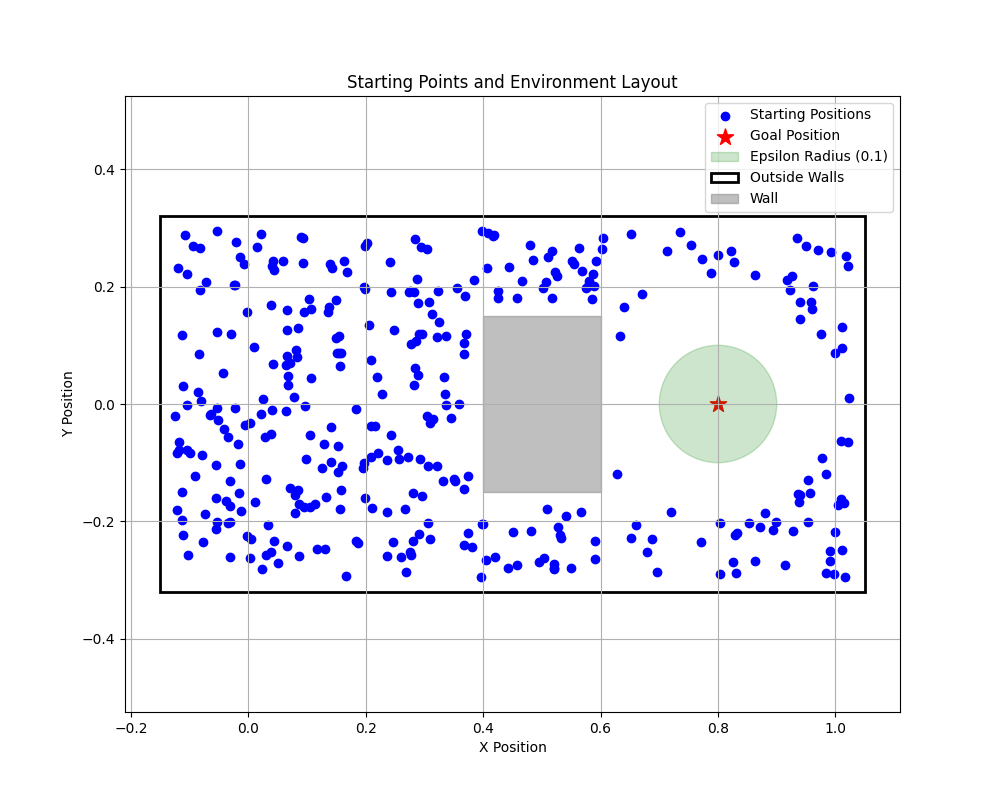
\includegraphics[width=0.82\textwidth]{images/gpu/spawns.png}
    \caption{Random collision-free training starts, obstacle geometry, and goal region.}
    \label{fig:ppo_spawns}
\end{figure}

\section{Hybrid Planning and Control}

\subsection{RRT Waypoints}
For every training or evaluation episode, an RRT is planned from the sampled start to the goal. The planner uses a step size of \(0.10\), a goal-sampling probability of \(0.20\), and at most \(1000\) iterations. Candidate points and segments are checked against the outer boundary and an inflated central obstacle. The resulting path is shortcut-smoothed and then densified so adjacent targets are no more than \(0.10\) apart. If the direct start-to-goal segment is collision-free, it is densified without growing a tree.

\subsection{PD Demonstrations}
The feedback expert generates bounded actions
\[
a_t^{\mathrm{PD}}=\tanh\!\left(
K_p(p_t^{\mathrm{wp}}-p_t)-K_d\dot{p}_t
\right),
\qquad K_p=6,\quad K_d=6.
\]
Before PPO begins, the actor is trained for \(30\) epochs on \(4096\) states sampled along collision-free RRT segments. This imitation stage gives the policy an initial obstacle-aware path-following behavior instead of requiring it to discover basic control entirely through sparse successes.

\subsection{Safety Shield}
The deployed control blends the policy and expert outputs:
\[
a_t^{\mathrm{safe}}=0.25a_t^{\pi}+0.75a_t^{\mathrm{PD}}.
\]
A one-step position prediction is checked against the environment with a \(0.025\) geometry clearance. If the prediction is unsafe, the shield substitutes the expert action. The final force is clipped component-wise to \([-1,1]\). The shield is used consistently during data collection, deterministic evaluation, and rendering.

\section{PPO Actor--Critic Model}

The actor and critic are separate fully connected networks with hidden widths \(32\), \(64\), and \(32\), ReLU activations, and Xavier initialization. The actor outputs the mean and standard deviation of a Gaussian distribution. The standard deviation is produced with a softplus function and constrained to \([0.05,0.5]\). A sampled raw action \(u_t\) is transformed with \(\tanh\) before it is sent to the safety shield. The critic estimates the scalar value \(V(o_t)\).

PPO uses the probability ratio
\[
r_t(\theta)=
\frac{\pi_\theta(u_t\mid o_t)}
     {\pi_{\theta_{\mathrm{old}}}(u_t\mid o_t)}
\]
and the clipped actor objective
\[
L_{\mathrm{actor}}=
-\mathbb{E}_t\left[
\min\left(
r_t\hat{A}_t,
\operatorname{clip}(r_t,1-\varepsilon_c,1+\varepsilon_c)\hat{A}_t
\right)\right],
\]
where \(\varepsilon_c=0.2\). Advantages are computed with generalized advantage estimation using \(\gamma=0.99\) and \(\lambda=0.95\), then normalized. The critic uses smooth \(L_1\) loss. The combined optimization objective includes a value coefficient of \(0.5\), entropy coefficient of \(0.01\), and gradient clipping at \(0.5\).

\section{Training}

Training runs for \(360\) episodes in batches of \(64\), with up to \(1800\) MuJoCo steps per episode. Each collected batch is optimized for six PPO epochs using minibatches of \(1024\) samples and an Adam learning rate of \(3\times10^{-4}\).

For a transition to next state \(s_{t+1}\), the implemented shaped reward is
\[
r_t =
-2d_{\mathrm{goal}}(s_{t+1})-0.01
+10\left(d_{\mathrm{wp}}(s_t)-d_{\mathrm{wp}}(s_{t+1})\right)
-2d_{\mathrm{cross}}(s_{t+1})
+100\,\mathbb{1}_{\mathrm{goal}}
-25\,\mathbb{1}_{\mathrm{collision}}.
\]
The terms penalize goal distance and elapsed time, reward progress toward the current waypoint, penalize cross-track error from the active path segment, reward goal entry, and strongly penalize collision. Episodes terminate on success, collision, or timeout.

After every training batch, the mean policy is evaluated without exploration on \(32\) newly sampled episodes. Checkpoint selection prioritizes lower collision rate, then higher success rate, and finally higher mean reward. Rendering loads this best checkpoint and uses deterministic mean actions.

\section{Results and Discussion}

\begin{figure}[H]
    \centering
    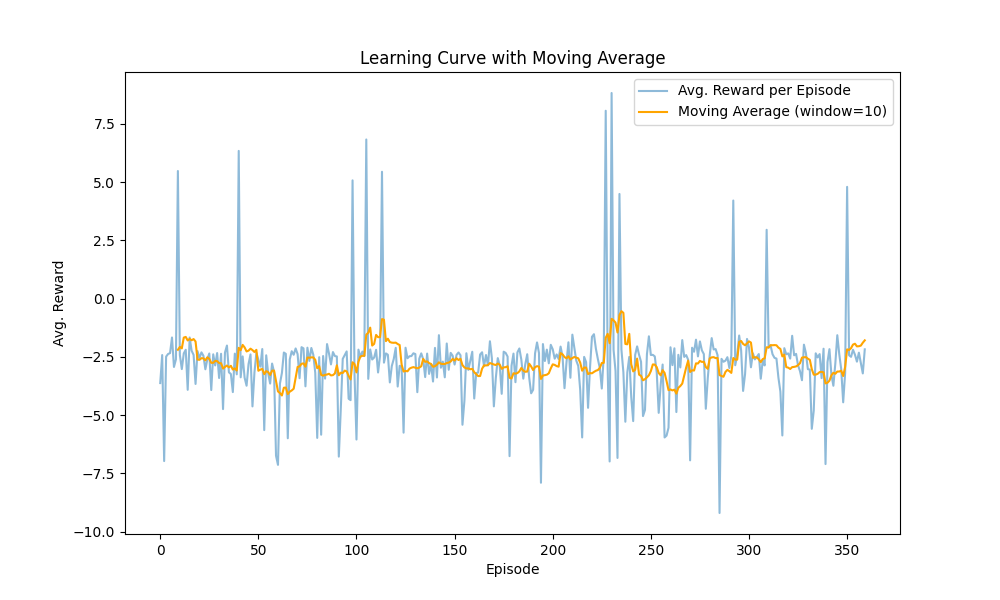
\includegraphics[width=0.82\textwidth]{images/gpu/leaning.png}
    \caption{Average training reward per episode and a ten-episode moving average over 360 episodes.}
    \label{fig:ppo_learning}
\end{figure}

The reward trace is noisy because episodes begin at different distances from the goal and PPO samples stochastic actions. Positive spikes correspond to successful episodes receiving the terminal bonus. The moving average remains mostly negative, so this plot alone does not demonstrate monotonic convergence; deterministic success and collision rates are the more meaningful checkpoint criteria.

\begin{figure}[H]
    \centering
    
\includegraphics[width=0.82\textwidth]{images/gpu/loss.png}
    \caption{Critic and clipped PPO actor losses during training.}
    \label{fig:ppo_losses}
\end{figure}

Most actor updates remain near zero because clipping limits large policy changes, with occasional spikes from batches containing unusually large normalized advantages. The critic also shows intermittent large errors associated with terminal rewards and variable episode outcomes. These traces support the use of gradient clipping and deterministic evaluation, but they should not be interpreted as proof of collision-free generalization.

The best saved checkpoint was selected after 64 training episodes. In its deterministic evaluation over 32 newly sampled episodes, it reached the goal in all 32 episodes and recorded no collisions. Its mean per-step reward was 0.6235. Table~\ref{tab:best_checkpoint} summarizes the checkpoint metadata stored with the model.

\begin{table}[H]
    \centering
    \begin{tabular}{lc}
        \hline
        \textbf{Metric} & \textbf{Best checkpoint} \\
        \hline
        Training episodes completed & 64 \\
        Deterministic evaluation episodes & 32 \\
        Success rate & 100\% \\
        Collision rate & 0\% \\
        Mean reward per step & 0.6235 \\
        \hline
    \end{tabular}
    \caption{Deterministic evaluation metrics stored in the best PPO checkpoint.}
    \label{tab:best_checkpoint}
\end{table}

\section{Conclusion}

The revised implementation is a hybrid collision-avoidance system rather than a standalone actor--critic agent. RRT provides route-level obstacle avoidance, PD imitation initializes and stabilizes waypoint tracking, PPO improves the stochastic policy, and the safety shield constrains executed actions. The separation of training, planning, environment, rendering, and plotting interfaces also makes the system easier to evaluate and extend. Future experiments should compare the learned policy against the expert-only controller, report confidence intervals across random seeds, and ablate RRT guidance, imitation pretraining, and the safety shield.

\begin{thebibliography}{9}
\raggedright

\bibitem{vanHasselt}
van Hasselt, H. Lecture 9: Policy Gradients and Actor Critics; UCL, 2021.

\bibitem{schulmanPPO}
Schulman, J.; Wolski, F.; Dhariwal, P.; Radford, A.; Klimov, O.
Proximal Policy Optimization Algorithms. arXiv:1707.06347, 2017.

\bibitem{schulmanGAE}
Schulman, J.; Moritz, P.; Levine, S.; Jordan, M.; Abbeel, P.
High-Dimensional Continuous Control Using Generalized Advantage Estimation.
arXiv:1506.02438, 2015.

\end{thebibliography}

\clearpage
\part{Kinodynamic RRT with PID Control}

\section{Introduction}
In robotics, autonomous path planning and control are crucial aspects of robot navigation, particularly in environments with obstacles. The objective of this project is to implement a hybrid approach that combines kinodynamic rapidly-exploring random Tree (RRT) for path planning and proportional-integral-derivative (PID) controllers for executing the motion along the planned path. This work is demonstrated using a ball in a MuJoCo simulation environment, where the ball navigates through an environment containing walls and boundaries. The goal is to move the ball from a starting position to a goal position while avoiding obstacles using the kinodynamic RRT algorithm and accurately controlling the movement with PID.

\subsection{Objectives}
The main challenge is efficiently generating a collision-free path from a start point to a goal point in a cluttered environment and ensuring the ball follows this path with minimal deviation. We undertook the following steps to achieve this objective:
\begin{itemize}
    \item Configuring MuJoCo and exploring various models, including Newton's cradle with no gravity.
    \item Developing basic pathfinding in a 3D environment using Dijkstra's algorithm for initial path selection and fixed velocity controls.
    \begin{figure}[h!]
        \centering
        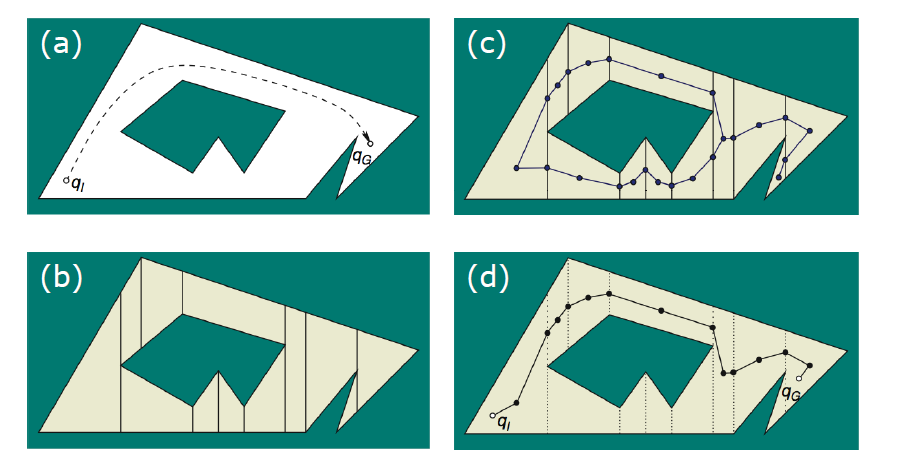
\includegraphics[width=0.5\textwidth]{images/rrt/trapezoidal.PNG}
        \caption{Trapezoidal decomposition (\(\mathcal{C} = \mathbb{R}^3_{\text{max}}\))\cite{mobile_robotics}}
        \label{fig:trapezoidal}
    \end{figure}
    \item Enhancing pathfinding with kinodynamic RRT, incorporating a safety margin around obstacles.
    \begin{figure}[h!]
        \centering
        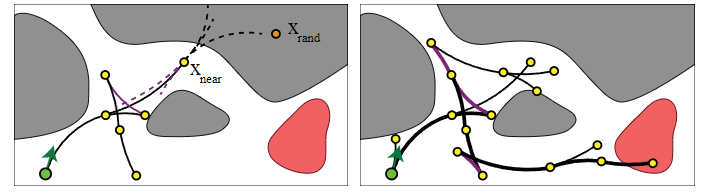
\includegraphics[width=0.5\textwidth]{images/rrt/kinodyanmics.PNG}
        \caption{Kinodynamic RRT}
        \label{fig:kinodynamic}
    \end{figure}
    \item Replacing basic controls with a PID controller to follow the planned path.
    \item Simulating and visualizing the robot's movement within the MuJoCo physics engine.
\end{itemize}

\section{Environment}
The environment consists of a 2D plane with predefined walls and boundaries. The simulation is conducted using the MuJoCo physics engine, which allows for the creation and control of dynamic models. For this project, a ball is moved through the environment containing a set of obstacles to reach the goal. The model used is defined in the \texttt{ball\_square.xml} file, and the walls are represented as both external boundaries and internal obstacles.

\subsection{Map}
\begin{itemize}
    \item \textbf{Dimensions:} The 2D environment spans from \(x = -0.5\) to \(x = 1.5\) and \(y = -0.4\) to \(y = 0.4\).
    \item \textbf{Obstacles:} A rectangular obstacle is placed in the middle of the environment between coordinates (0.5, -0.15) and (0.6, 0.15), acting as a wall.
    \item \textbf{Goal Area:} The target area for the robot is set between coordinates (0.9, -0.3) and (1.1, 0.3).
    \item \textbf{Boundaries:} The outer walls of the environment prevent the robot from moving outside the area.
\end{itemize}

\begin{figure}[h]
    \centering
    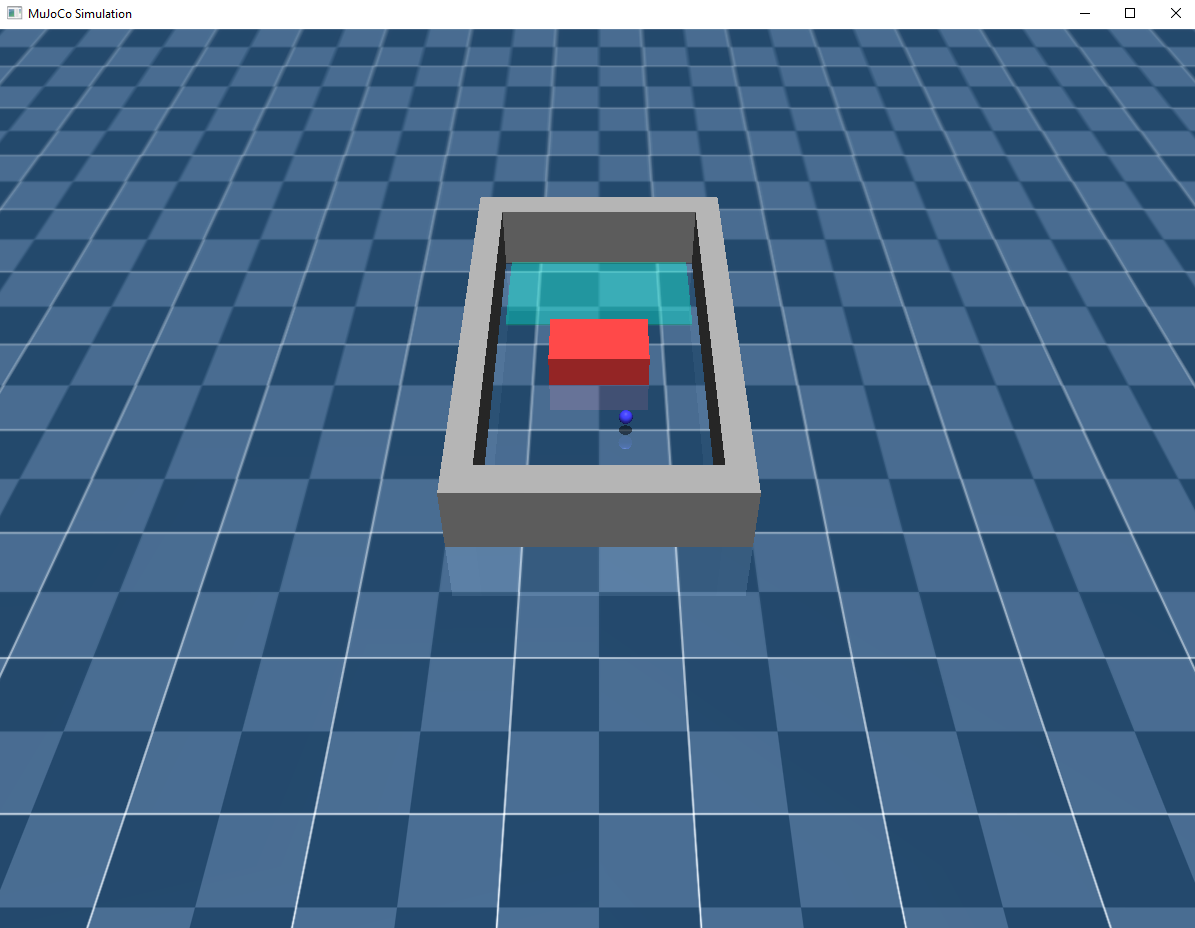
\includegraphics[width=0.5\textwidth]{images/rrt/render.PNG}
    \caption{Environment Setup}
    \label{fig:environment}
\end{figure}

This setup ensures the presence of both static and dynamic constraints, making path planning non-trivial and control challenging.

\section{Path Planning}

\subsection{Algorithm Overview}
RRT\cite{planning_dynamics} is widely used for motion planning in high-dimensional spaces. In this project, we implement a kinodynamic variant of RRT. Unlike standard RRT, the kinodynamic RRT accounts for the robot's dynamics while generating the tree, ensuring that the planned path can be followed realistically by the robot. This approach helps avoid sharp or unrealistic turns that the robot may not be able to follow.

The algorithm grows a tree from the start position by:
\begin{enumerate}
    \item Sampling a random point in the environment.
    \item Identifying the nearest node in the tree.
    \item Applying a control input to move the robot towards the sampled point, simulating its dynamics.
    \item Checking the resulting position for collisions.
    \item Adding the new position to the tree if no collision occurs.
\end{enumerate}

This process repeats until the robot reaches the goal area or a maximum number of iterations is reached. The function \texttt{kinodynamic\_rrt} implements this process, while \texttt{simulate} handles the forward simulation of the robot's dynamics.
    
\begin{figure}[h]
    \centering
    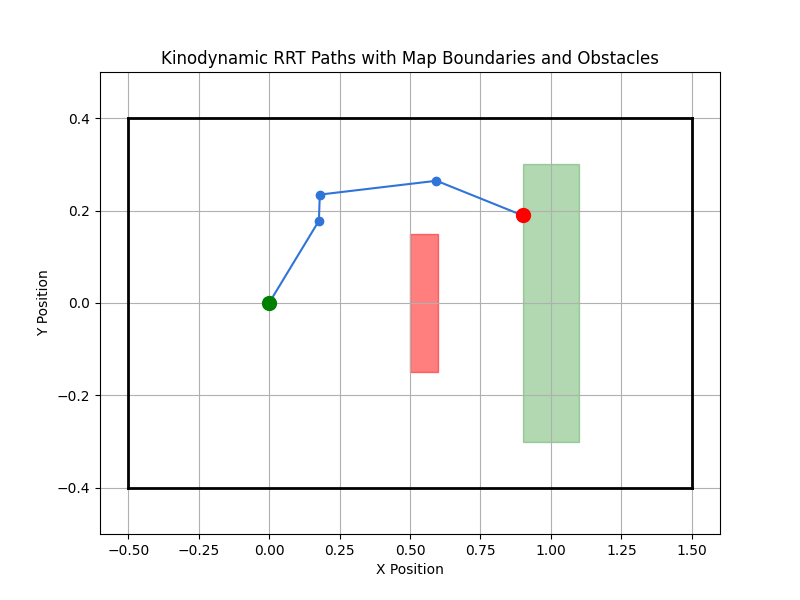
\includegraphics[width=0.5\textwidth]{images/rrt/path.png}
    \caption{Kinodynamic RRT}
    \label{fig:sample_image}
\end{figure}

\subsection{Purpose of \texttt{simulate()} in \texttt{kinodynamic\_rrt}}
In traditional RRT, paths are generated based solely on geometric feasibility. However, for real systems with dynamic constraints, \texttt{simulate()} serves several critical functions:
\begin{itemize}
    \item \textbf{Ensures Dynamic Feasibility:} Calculates movement towards each sampled point, adjusting with PID control.
    \item \textbf{Incremental Adjustment:} Makes small, corrective adjustments to follow a feasible path.
    \item \textbf{Collision-Free Verification:} Confirms both geometric and dynamic feasibility.
    \item \textbf{Realistic Path Execution:} Validates that each RRT segment can be executed under real-world constraints.
\end{itemize}
    
\subsection{Collision Avoidance}
Collision detection is handled by the function \texttt{is\_collision\_free}, which checks if the robot's new position lies within any of the obstacle regions or the environment boundaries. A safety margin is applied to ensure that the robot does not approach obstacles too closely. The function \texttt{is\_collision\_free\_line} checks if a straight line between two points is free of obstacles by verifying that there are no collisions with specified walls.

\subsection{Path Construction}
Once the algorithm successfully identifies a path to the goal, the tree is traversed from the goal node back to the start node to construct the complete path. This backtracking process is handled by the function \texttt{construct\_path}. The final path is then visualized, displaying the trajectory, environmental boundaries, and any obstacles encountered along the way.

When a path is established between two nodes, the function \texttt{line\_goes\_through\_goal} checks if the path intersects with the goal area by interpolating and sampling points along the path. If an intersection is detected, the endpoint is adjusted to the coordinates (0.9, y) based on the last generated point. This modification effectively minimizes the distance required to reach the goal, as evidenced by the time trial paths.

\subsection{Smoothing}
After selecting the path within the Rapidly-exploring Random Tree, post-processing occurs using the \texttt{smooth\_path} function. This function randomly selects points in the graph to determine if they can be directly connected while eliminating intermediate points. As a result, the path is reduced to a series of critical waypoints, simplifying navigation. This reduction allows the control implementation to restart upon reaching each subsequent point, providing the controller with adequate time to complete the feedback loop before moving on to the next waypoint.

\section{Navigation}

\subsection{Controller}
PID controllers are commonly used in control systems to achieve stable and accurate control. In this project, two PID controllers are implemented: one for controlling the movement of the ball in the \(x\)-direction and the other for the \(y\)-direction. Each controller computes the control input based on the error between the current and target positions, aiming to reduce this error over time.

The function \texttt{move\_ball\_to\_position\_with\_pid} implements the control loop, where the ball's current position is compared to the target position from the planned path. The PID controllers compute the necessary force to move the ball toward the target, and the control inputs are applied in each iteration of the simulation.

\begin{equation}
u(t) = K_p e(t) + K_i \int_0^t e(\tau) \, d\tau + K_d \frac{d}{dt} e(t)
\end{equation}

where:
\begin{itemize}
    \item \( K_p \): Proportional gain,
    \item \( K_i \): Integral gain,
    \item \( K_d \): Derivative gain,
    \item \( e(t) = r(t) - y(t) \): Error at time \( t \).
\end{itemize}

\subsection{Parameters}
The gains for the PID controllers were manually tuned to achieve smooth movement without overshooting. This tuning required observing the patterns in the model simulation and adjusting accordingly; no penalty for previous errors was applied. The proportional (\texttt{kp}), integral (\texttt{ki}), and derivative (\texttt{kd}) gains were set as follows:
\begin{itemize}
    \item \textbf{Proportional Gain (\texttt{kp}):} 0.58---provides a basic correction based on the current error.
    \item \textbf{Integral Gain (\texttt{ki}):} 0---not used in this implementation to avoid cumulative errors from drift.
    \item \textbf{Derivative Gain (\texttt{kd}):} 0.5---helps to smooth the response by anticipating future errors based on the rate of change.
\end{itemize}

The higher proportional gain results in more aggressive error correction, which was necessary to achieve trials below a certain time threshold. Once the new point is set, the ball minimizes the error by updating its velocity. The \(x\)-direction and \(y\)-direction have the same controller configuration for symmetry. The same controllers are used to simulate the motion planning between two nodes in the Rapidly-exploring Random Tree.

\subsection{Pathfinder}
The PID controllers move the ball sequentially through each point in the planned path. Movement is clamped to prevent overshooting, and the simulation continues until the ball reaches the goal position with minimal error (set to 0.075 in this case). 

\begin{figure}[h!]
    \centering
    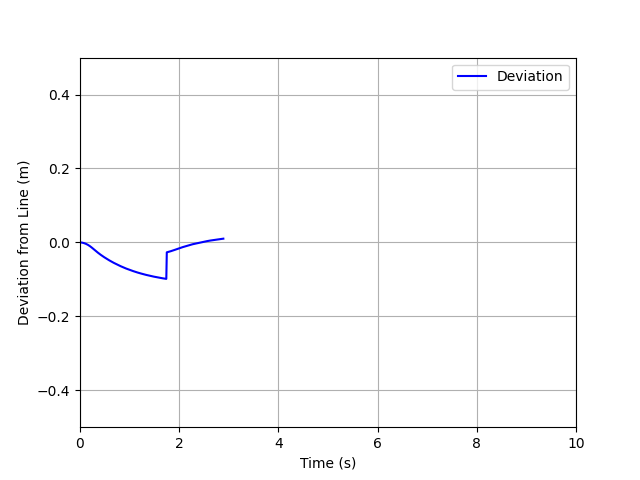
\includegraphics[width=0.5\textwidth]{images/rrt/deviation.png}
    \caption{Path Deviation}
    \label{fig:path_deviation}
\end{figure}
 
The deviation is calculated using the \texttt{calculate\_deviation} function. This feedback is important for determining how far the ball is from the trajectory, what adjustments to the controllers are necessary, and ensuring that the ball will not collide with obstacles between two points.

\subsection{Adjustments}

Several challenges arise during the control process, including handling sharp turns in the path and adjusting the control parameters to prevent oscillations. The derivative gain plays a crucial role in damping the response and ensuring smooth transitions between points. The best method for finding the right parameter was increasing the $K_p$ value until oscillation was guaranteed. The Ziegler--Nichols tuning method \cite{ziegler-nichols-wiki} is a heuristic approach to tuning a PID controller, developed by John G. Ziegler and Nathaniel B. Nichols. It is used to determine the proportional, integral, and derivative gains \( K_p \), \( K_i \), and \( K_d \) for a PID controller.

\begin{table}[h!]
    \centering
    \begin{tabular}{|c|c|c|c|}
        \hline
        \textbf{Controller Type} & \( K_p \) & \( K_i \) & \( K_d \) \\
        \hline
        P & \( 0.5 K_u \) & - & - \\
        PI & \( 0.45 K_u \) & \( \frac{K_p}{0.83 T_u} \) & - \\
        PD & \( 0.8 K_u \) & - & \( K_p \cdot 0.125 T_u \) \\
        PID & \( 0.6 K_u \) & \( \frac{K_p}{0.5 T_u} \) & \( K_p \cdot 0.125 T_u \) \\
        \hline
    \end{tabular}
    \caption{Ziegler--Nichols Tuning Parameters}
    \label{tab:zn_parameters}
\end{table}

\subsection{Path Visualization and Obstacle Mapping}
The function \texttt{visualize\_final\_tree} generates a graphical representation of the kinodynamic RRT, illustrating the exploration process and highlighting the path to the goal. The easiest approach to path visualization was created a top down $2D$ view for visualizing the path on the map. This perceptive aided the team in debugging how the path was getting created, the optimal path, and dangers in specific areas. As an example, the $2d$ view showed that the ball was getting too close to the front of the obstacle. Based on the limited controls and the time constraints, the ball would get too close and not know how to get out of the situation. The new information allowed use to implement a buffer around the object preventing the path from entering that area. 

\subsection{Dynamic Speed Adjustment for Smooth Deceleration}
The function \texttt{update\_speed} adjusts the robot's speed based on its distance from the goal, allowing for controlled deceleration to avoid overshooting.

\section{Results}

There were three main objectives in this experiment. The first one was getting the environment running, the second generating a path using kinodynamic RRT, and the third was getting the ball to the goal using controllers. The team demonstrated success on all three objectives. 

\subsection{Environment}

The model creation and execution worked well in the MuJoCo environment and allowed the team to witness the controller behavior prior to using in the kinodynamic RRT search. The simulated search for the path should reflect accuracy how the ball would actually move in the space to the way points and maintain control. It prevented the team was implement controller that behave erratically and would not lead to generating a complete path.

\subsection{Visualize Trees}

At the end of the report, a complete tree generated using kinodynamic RRT used as a path to the goal. The trees show the effectiveness of using kinodynamic RRT and the success rate for finding the goal despite the different seed. In trails 2, 4, and 5, the tree is not expansive showing the quickness for finding a node in the goal. An area worth exploring in the future is implement a suite of controllers and randomly selecting them for a better representation. In this experiment, the team is using one controller for all the path finding. 

\subsection{Time Trials}

The \texttt{run\_planning\_trial} function runs multiple trials and evaluates the success rate of the kinodynamic RRT in reaching the goal area in the a defined time limit. The team was successful in getting a path each trail and under the time contraints with a $100\%$ accuracy. The quickest shows the effectiveness for using a PID controller for path finding and simulating the ball movements to better represent the actual movement. Similar to the drone movement in the University of Utah technical report \cite{uucs_12_002}, kinodynamic RRT is a reasonable approach for solving this problem. 

\begin{figure}[h!]
    \centering
    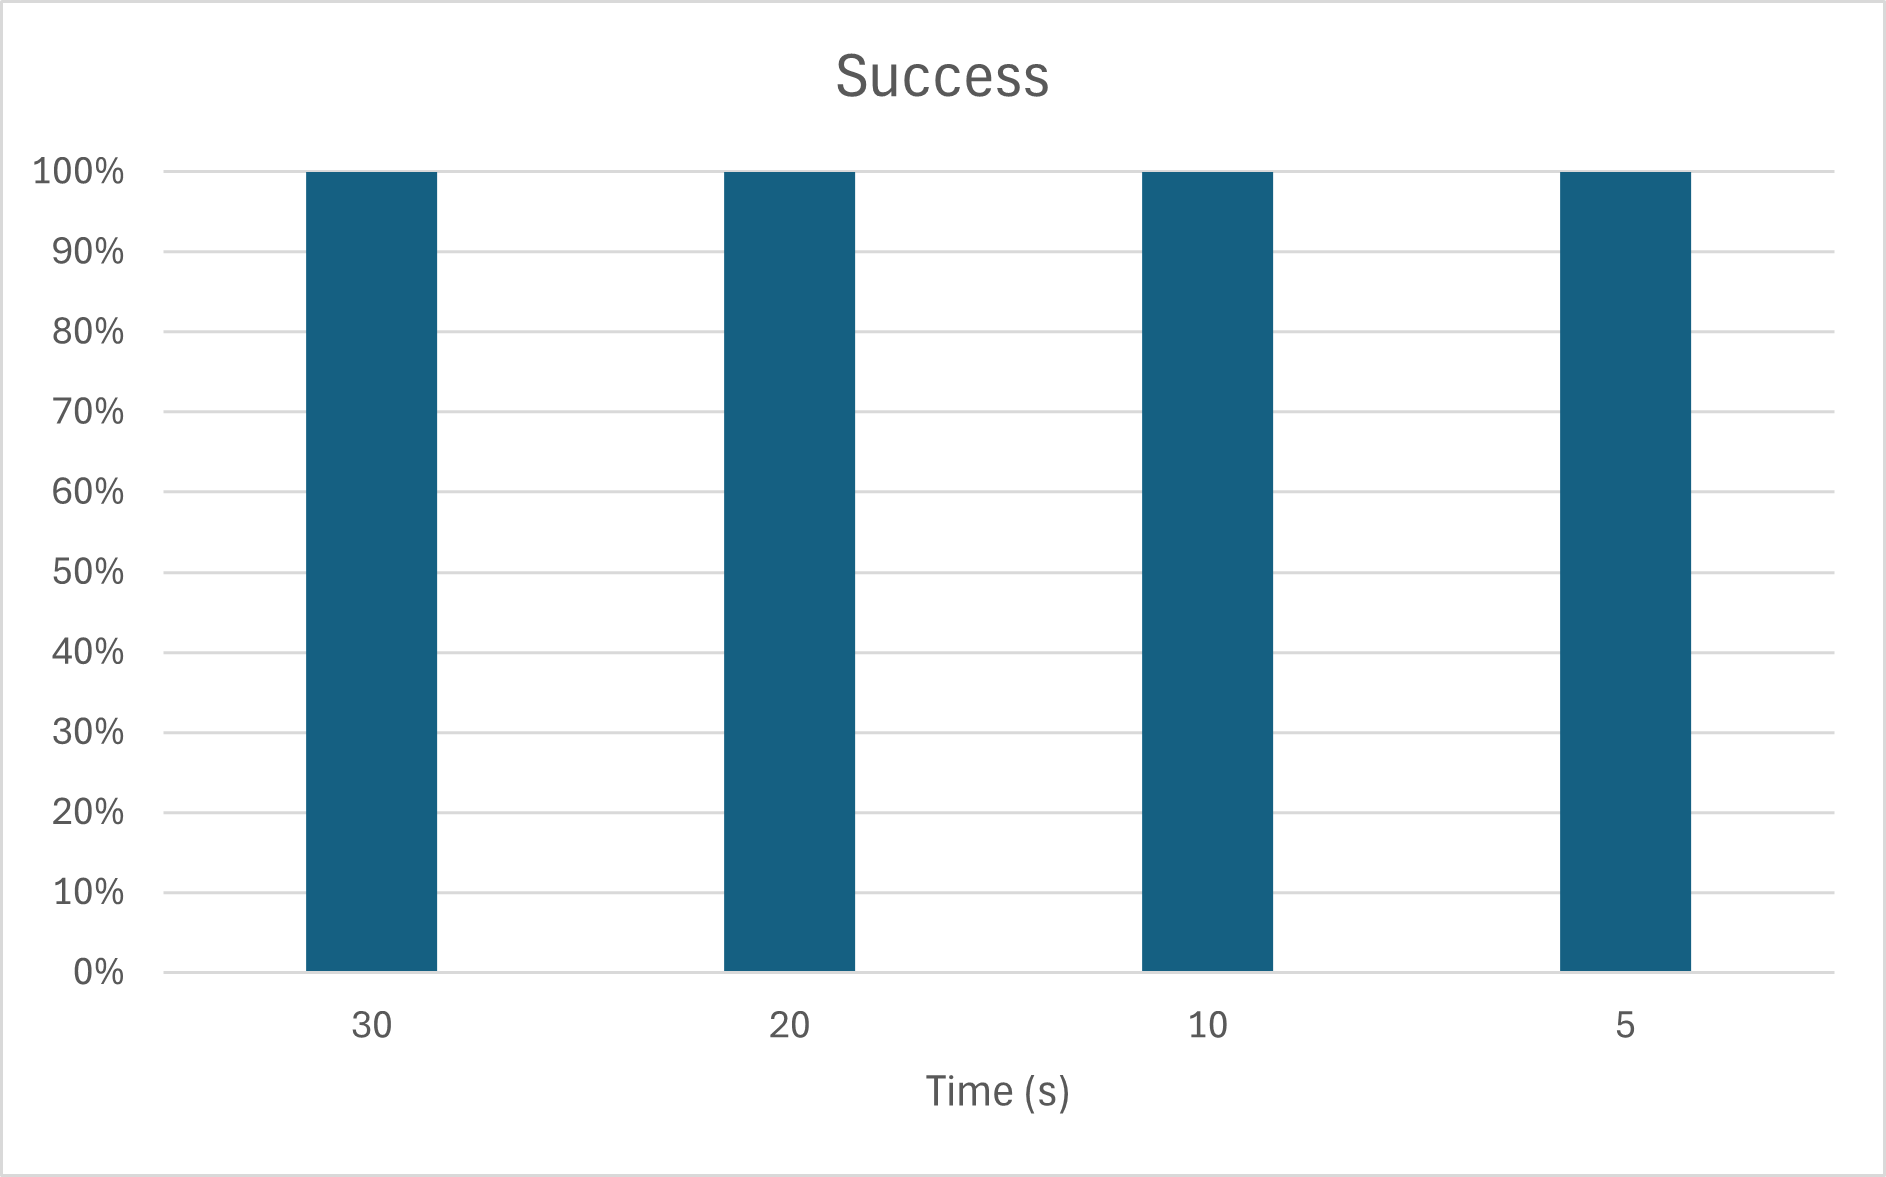
\includegraphics[width=0.5\textwidth]{images/rrt/success.png}
    \caption{Success Rates}
    \label{fig:success_rates}
\end{figure}

\section{Conclusion}
This project successfully integrated kinodynamic RRT for path planning and PID control for path execution in a simulated 3D environment. By leveraging these techniques, ball can navigate a complex environment with obstacles and boundaries while accurately following the planned path to the goal.

\begin{thebibliography}{}
\raggedright

\bibitem{mobile_robotics}
Burgard, Wolfram, et al. Introduction to Mobile Robotics. Slides by Kai Arras, last updated July 2011, with material from S. LaValle, J.C. Latombe, H. Choset, and W. Burgard. \href{http://ais.informatik.uni-freiburg.de/news/index_en.php}{http://ais.informatik.uni-freiburg.de/news/index\_en.php}

\bibitem{planning_dynamics}
Planning with Dynamics and Uncertainty. \href{https://motion.cs.illinois.edu/RoboticSystems/PlanningWithDynamicsAndUncertainty.html}
{https://motion.cs.illinois.edu/RoboticSystems/PlanningWithDynamicsAndUncertainty.html}

\bibitem{uucs_12_002}
University of Utah, School of Computing. Technical Report UUCS-12-002, 2012. \href{https://www-old.cs.utah.edu/docs/techreports/2012/pdf/UUCS-12-002.pdf}{https://www-old.cs.utah.edu/docs/techreports/2012/pdf/UUCS-12-002.pdf}

\bibitem{ziegler-nichols-wiki}
Wikipedia contributors, "Ziegler--Nichols method," \textit{Wikipedia},
\url{https://en.wikipedia.org/wiki/Ziegler%E2%80%93Nichols_method}, accessed 26-October-2024.

\end{thebibliography}

\begin{figure}[h!]
    \centering
    \begin{subfigure}{0.45\textwidth}
        \centering
        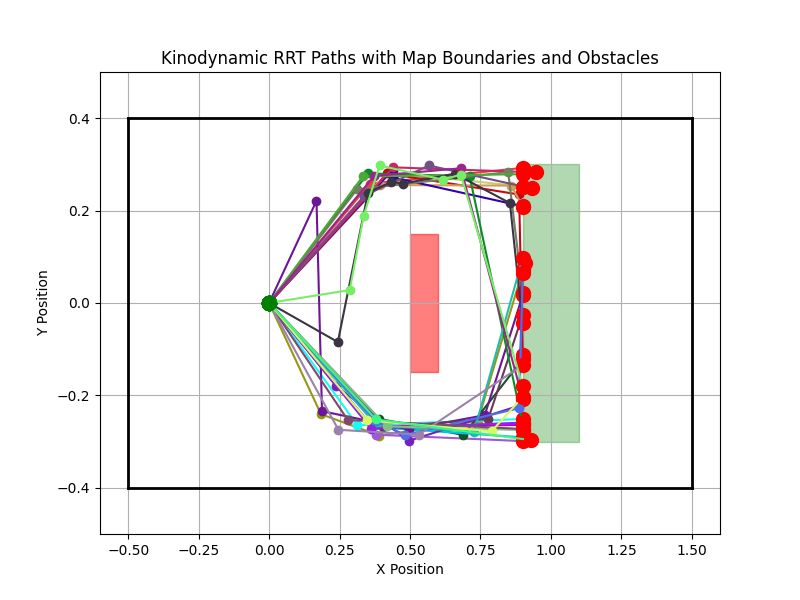
\includegraphics[width=\textwidth]{images/rrt/5.png}
        \caption{Tmax = 5}
        \label{fig:5.png}
    \end{subfigure}
    \hfill
    \begin{subfigure}{0.45\textwidth}
        \centering
        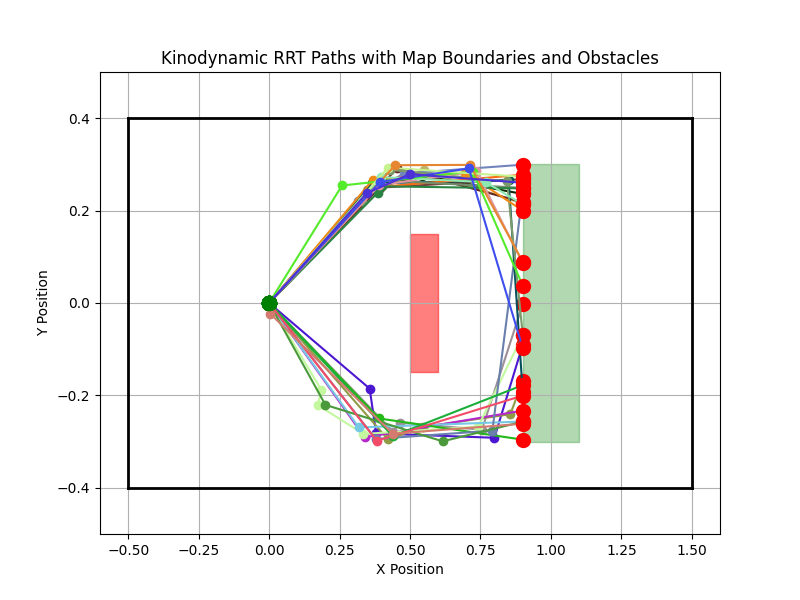
\includegraphics[width=\textwidth]{images/rrt/10.png}
        \caption{Tmax = 10}
        \label{fig:10.png}
    \end{subfigure}
    
    \vspace{0.5cm} % Adds some vertical space between rows

    \begin{subfigure}{0.45\textwidth}
        \centering
        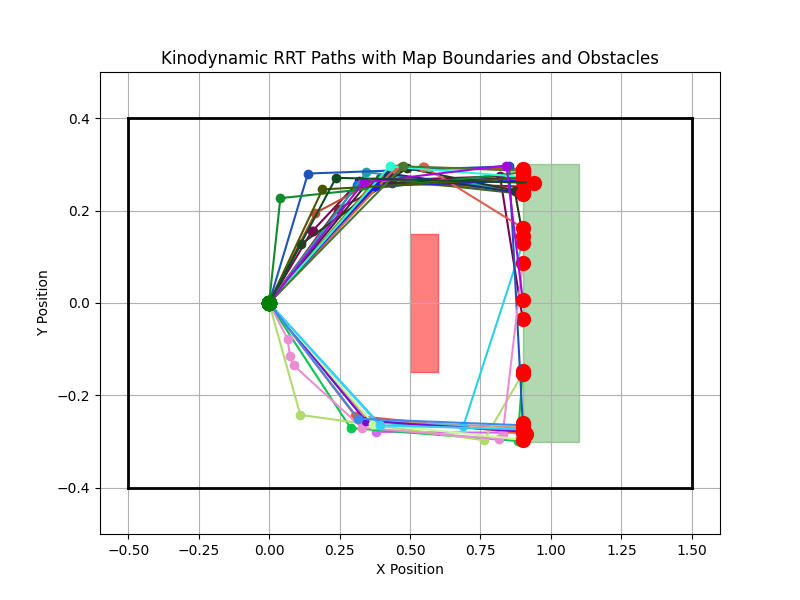
\includegraphics[width=\textwidth]{images/rrt/20.png}
        \caption{Tmax = 20}
        \label{fig:20.png}
    \end{subfigure}
    \hfill
    \begin{subfigure}{0.45\textwidth}
        \centering
        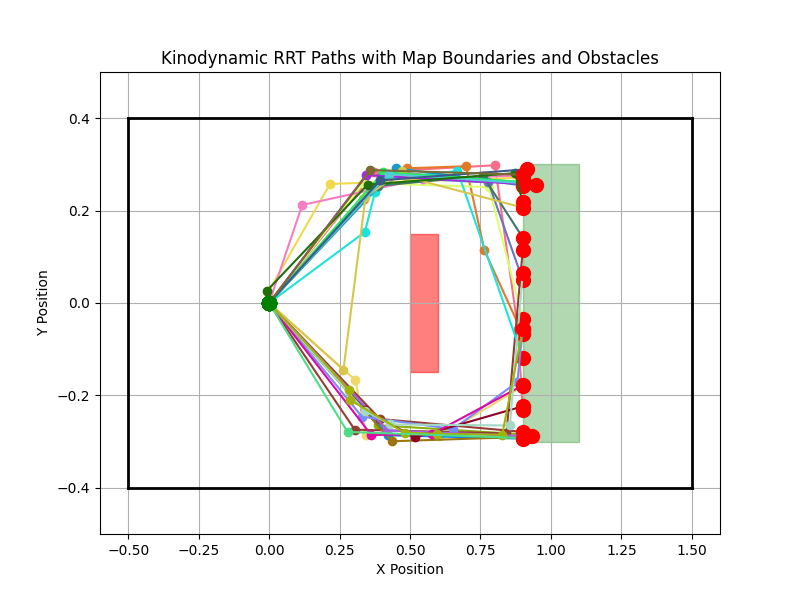
\includegraphics[width=\textwidth]{images/rrt/30.png}
        \caption{Tmax = 30}
        \label{fig:30.png}
    \end{subfigure}

    \caption{Visualization of path exploration}
    \label{fig:time_trials}
\end{figure}

\begin{figure}[h!]
    \centering
    \begin{subfigure}{0.45\textwidth}
        \centering
        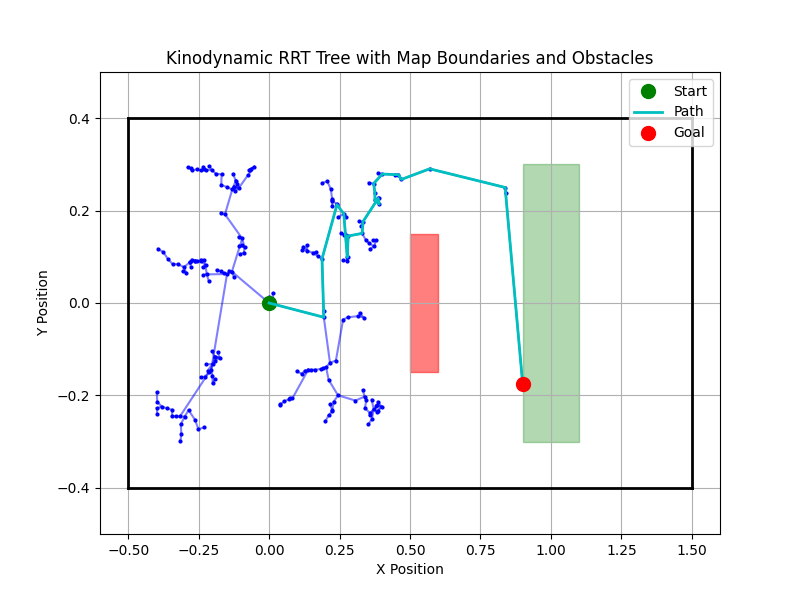
\includegraphics[width=\textwidth]{images/rrt/tree1.png}
        \caption{Trial 1}
        \label{fig:tree_1}
    \end{subfigure}
    \hfill
    \begin{subfigure}{0.45\textwidth}
        \centering
        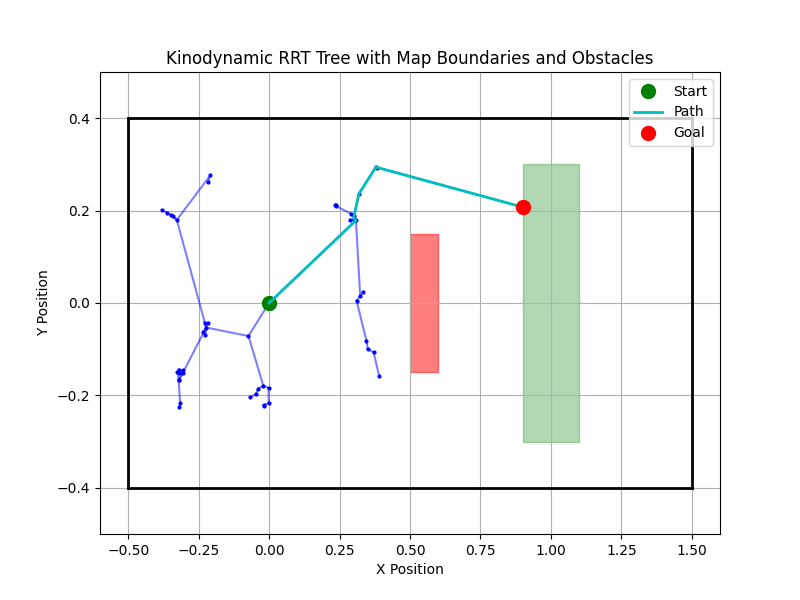
\includegraphics[width=\textwidth]{images/rrt/tree2.png}
        \caption{Trial 2}
        \label{fig:tree_2}
    \end{subfigure}
    
    \vspace{0.5cm} % Adds some vertical space between rows

    \begin{subfigure}{0.45\textwidth}
        \centering
        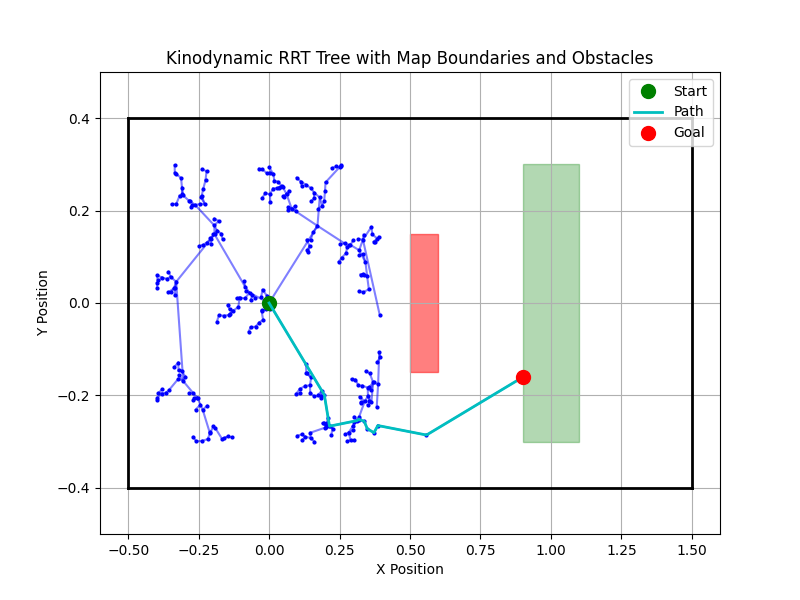
\includegraphics[width=\textwidth]{images/rrt/tree3.png}
        \caption{Trial 3}
        \label{fig:tree_3}
    \end{subfigure}
    \hfill
    \begin{subfigure}{0.45\textwidth}
        \centering
        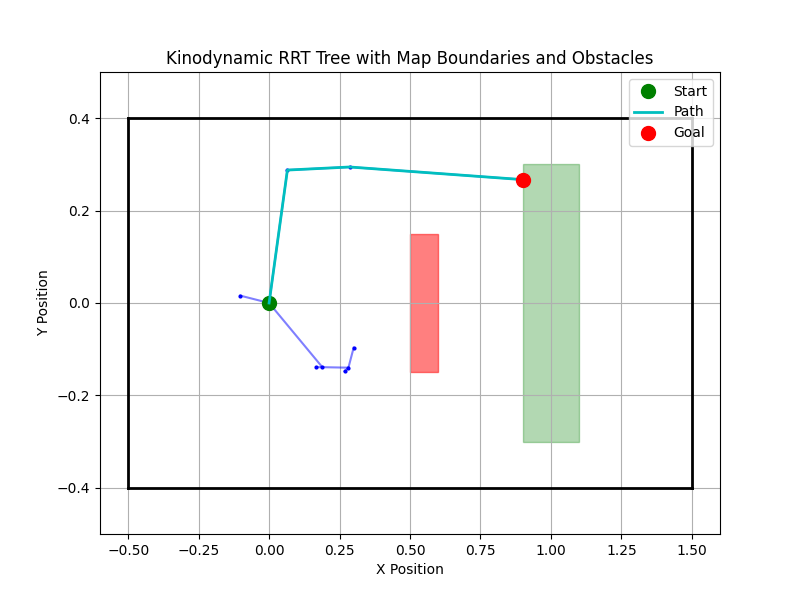
\includegraphics[width=\textwidth]{images/rrt/tree4.png}
        \caption{Trial 4}
        \label{fig:tree_4}
    \end{subfigure}

    \begin{subfigure}{0.45\textwidth}
        \centering
        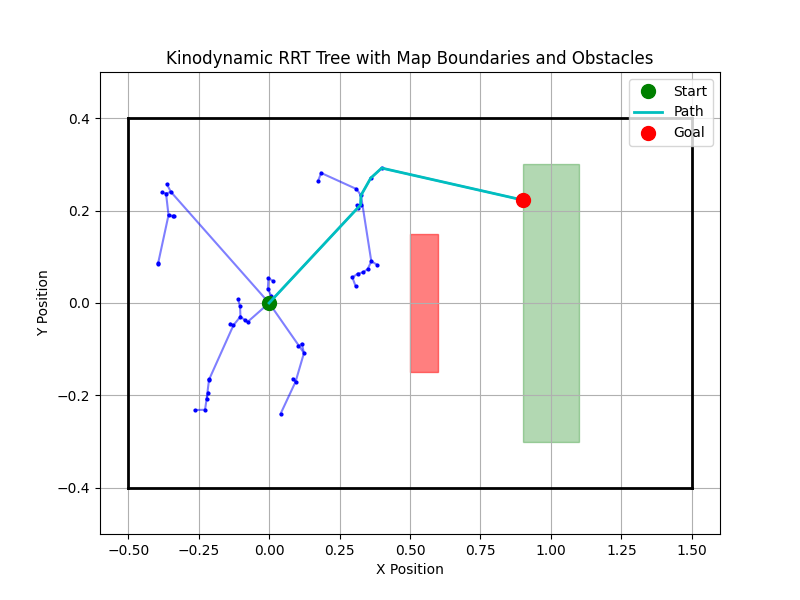
\includegraphics[width=\textwidth]{images/rrt/tree5.png}
        \caption{Trial 5}
        \label{fig:tree_5}
    \end{subfigure}

    \caption{Visualization of trees for different trials.}
    \label{fig:trials}
\end{figure}

\end{document}
